\documentclass{article}
\usepackage{graphicx}
\usepackage{hyperref}
\usepackage{listings}
\usepackage{float}
\usepackage[margin=1in]{geometry}

\title{Horizontal scaling of streaming applications on Kubernetes.}
\author{Mikołaj Nowak 184865 \and Jakub Waśniewski 184943}
\date{}

\begin{document}

\maketitle

\section{About the project}\label{about-the-project}

The goal of this project is to show different conceptions and approaches regarding:
\begin{itemize}
  \item VOD streaming with various protocols, especially HTTP-based ones like HLS and MPEG-DASH
  \item Advantages of HLS and MPEG-DASH such as Adaptive Bitrate Streaming
  \item Creating streams with ffmpeg solution
  \item Kubernetes, including its architecture, our infrastructure, and horizontal scaling
\end{itemize}

\section{Setup}\label{setup}

In order to run this project follow these steps:
\begin{enumerate}
    \item Download and install \href{https://ffmpeg.org}{ffmpeg}.
    
    \item If you'd like to stream your custom video, prepare or download an appropriate .mp4 file. For example, you can download the full BigBuckBunny 10 minutes movie from \href{http://commondatastorage.googleapis.com/gtv-videos-bucket/sample/BigBuckBunny.mp4}{here}. If not, you can use the Sintel Trailer (sinteltrailer.mp4 file) provided by default.
    
    \item Place the .mp4 file in the \emph{apps/streaming-server/} directory.
    
    \item In the \emph{apps/streaming-server/} directory, run: \texttt{./convert.sh -i MY\_MOVIE\_FILE.mp4}.
    
    \item If you're on a Windows machine, you can either configure WSL or use a faster workaround by downloading \href{https://git-scm.com/downloads}{GIT}. After downloading it, you can run the script from GIT Bash as mentioned above, or add a path to sh.exe file (for example, \emph{C:\textbackslash Program Files\textbackslash Git\textbackslash bin}) to the PATH variable and run it from PowerShell like \texttt{sh .\textbackslash convert.sh -i MY\_MOVIE\_FILE.mp4}.
    
    \item To run this app, you need to have a prepared Kubernetes cluster. The easiest way to provide it is to run a local one-node cluster called \texttt{minikube}. To do that, download minikube and start it with \texttt{minikube start}.
    
    \item Deploy the application by using the script shown below. Give it some time to properly deploy all apps on the cluster, and you're ready to go.

    \begin{verbatim}scripts/build_images_and_deploy.sh --rebuild-images --deploy-streaming-server\end{verbatim}
    
    \item Use 
    \begin{verbatim}minikube service streaming-server-service -n streaming-service \end{verbatim}
      to access an application in a browser. It will automatically redirect
      you to the browser. If not - copy the printed IP with port and paste
      it in the browser.
    \item
      To simulate a workload on a web app use
      \begin{verbatim}kubectl apply -f k8s/helpers/web-load-generator.yaml\end{verbatim}
      After that you will see HPA automatically deploying all replicas
      across the node.
    \item
      Optionally, if you have Docker installed on your machine and you'd
      like to run simple streaming-server Docker container without any
      Kubernetes you can run: \texttt{./init-pure-docker.sh} in the
      \emph{streaming-server/} directory and visit the application on
      \href{http://localhost:8080}{http://localhost:8080}.
\end{enumerate}

\section{Streaming - theoretical
introduction}\label{streaming---theoretical-introduction}

Before we get into the details of how our streaming application works,
let's first discuss the basics of streaming, its definition, a brief
history and the appropriate protocols.

\subsection{What is streaming?}\label{what-is-streaming}

In simple words streaming, or more specifically, streaming media, is the continuous delivery of multimedia
content from a server to a client with little or no intermediate storage of the data.

We can distinguish two ways of accessing streaming data: live and
on-demand. In our project, we will focus on on-demand access,
specifically in the form of VOD (Video on Demand). 
The most popular services of this type include Netflix, HBO Max, Hulu, and Disney Plus.

\subsection{A brief history of
streaming}\label{a-brief-history-of-streaming}

\subsubsection{Downloading}\label{downloading}

Downloading is the oldest way of offering video and has little to do
with today's streaming. Due to the fact that the meta data summary was
located at the end of a media file, the entire file would need to be
downloaded in order for the meta data to be read and the player begin
playback.

\subsubsection{Progressive download}\label{progressive-download}

After relocating the metadata from the end to the beginning of the
digital media file, the media player obtained all the necessary
information to initiate playback while the file was still being
downloaded. This provided an experience similar to today's streaming,
but it represents an old method of delivering video, and the basic
version of progressive download lacks many functionalities that we
commonly find in modern streaming. There have been some improvements to
progressive download that make it resemble streaming to a certain
extent, this improved version of progressive download is often referred
to as pseudostreaming. However, even with these improvements, there is
still a significant disadvantage that cannot be overlooked: with
progressive download, the file is downloaded to a physical drive on the
end user's device, which is undesirable from a copyright perspective.

It's worth to mention that progressive download is natively supported in
HTML5 player.

\subsubsection{RTMP}\label{rtmp}

RTMP serves as a communication protocol designed for the streaming of
audio, video, and data across the Internet. Initially created as a
proprietary protocol by Macromedia to facilitate streaming between Flash
Player and the Flash Communication Server, however Macromedia was later
acquired by Adobe along with the rights to RTMP protocol.

RTMP was the leading streaming protocol in the mid-2000s. Its major
advantage was the widespread installation of Adobe Flash Player, which,
as we all know, is no longer the case. Another significant advantage of
RTMP is its low latency.

However, it also comes with several disadvantages, such as security
issues associated with Adobe Flash Player, the fact that it was
proprietary, its inability to leverage HTTP-based infrastructure, and
its unsuitability for \texttt{Adaptive\ Bitrate\ Streaming\ (ABR)} which
is dynamically adapting content quality to user's bandwith or caching at
edge locations with a CDN (Cloud Delivery Network), which significantly
enhances the performance of modern streaming.

Even though RTMP is not used when communicating between media server and
players due to the lack of Adobe Flash Player in our browsers, it still
can and is sometimes used in communication between source encoders and
media server.

\subsubsection{HLS}\label{hls}

HLS, or HTTP Live Streaming, stands as an HTTP-centric streaming
protocol introduced by Apple in 2009. Widely adopted, supported by many
media players, web browsers, mobile devices, and streaming media
servers. According to
\href{https://bitmovin.com/wp-content/uploads/2022/12/bitmovin-6th-video-developer-report-2022-2023.pdf}{bitmovin
yearly surveys} it's currently most popular streaming format.

Let's talk a bit about how HLS works. Content, for example some movie,
is divided into small chunks, each has a few seconds of video and audio.
A manifest file, also knows as playlist file, provides the list of all
chunks and some additional data. Manifest and chunks can de either
pre-processed (like with movie example) or prepared upon request. First
approach is more popular in VOD streaming and second one can be used
when we have single live streaming source that can utilize RTMP protocol
and then we take this RTMP stream and convert it to HLS stream which can
then be delivered directly to the end users (or to their player to be
specific).

In HLS the manifest is stored in a file with the .m3u8 extension, which
is commonly used for M3U playlist files in the UTF-8 (Unicode) format.
Individual segments by default has .ts extension.

HLS supports \texttt{Adaptive\ Bitrate\ Streaming\ (ABR)} and caching at
edge locations with a CDN.

\subsubsection{MPEG-DASH}\label{mpeg-dash}

MPEG-DASH is similar to HLS when it comes to the principle of operation.
In MPEG-DASH content is also divided into small chunks but with the .m4s
extension and the playlist is a bit more complex and has XML format and
.mpd extension. MPEG-DASH also supports ABR and CDN. There are however
some differences between HLS and MPEG-DASH: - HLS is often natively
supported by Apple devices, MPEG-DASH is not. - default segment duration
in HLS is 6 seconds but it can be changed which is especially used in
LL-HLS (Low Latency HLS), optimal segment duration in MPEG-DASH is 2-4
seconds. - HLS is Apple proprietary protocol and MPEG-DASH is an
international standard (ISO/IEC 23009-1:2022) - the biggest advantage of
MPEG-DASH over HLS is a fact that MPEG-DASH is codec agnostic. It means
that it supports any codec standard, meanwhile HLS supports only H.264
and H.265 video encoding and small number of audio encoding standards.
Due to this and the previous reason MPEG-DASH is becoming increasingly
popular

\section{Streaming application
implementation}\label{streaming-application-implementation}

In this section, we will get into the practical aspects of our project
in order to provide a clear understanding of HTTP-based streaming protocols
like HLS and MPEG-DASH. We'll compare these protocols with progressive
downloading and highlight the significance of Adaptive Bitrate Streaming
(ABR). We'll divide this section based on certain components of our
streaming application and software, tools, solutions etc. that we used.

\subsection{Streams creation}\label{streams-creation}

In order to create appropriate HLS and MPEG-DASH streams we used FFmpeg.
FFmpeg is a complete, cross-platform solution to record, convert and
stream audio and video. We created the manifest file and chunks based on
.mp4 file which is a multimedia container format, containing video,
audio and also other data such as subtitles, metadata and still images.
It support various codecs, for example H.264 for video, AAC for audio
and MPEG-4 Timed Text for subtitles.

\subsubsection{HLS}\label{hls-1}

Here are the ffmpeg command that we used in order to create HLS stream:

\begin{verbatim}
# HLS
ffmpeg -i $INPUT_FILE \
  -vcodec libx264 \
  -acodec aac \
  -start_number 0 \
  -hls_time 3 \
  -hls_list_size 0 \
  -f hls $OUTPUT_PATH/hls/hls-stream.m3u8
\end{verbatim}

Let's describe each HLS converting option one by one:

\begin{itemize}
    \item \texttt{-i \$INPUT\_FILE}: Specifies the input file or stream for conversion. As mentioned in previous sections, it does not have to be an .mp4 file like in our example; you can use, for example, an RTMP stream as input.
    
    \item \texttt{-vcodec libx264}: Specifies the video codec to H.264. Keep in mind that HLS only supports H.264 and H.265 video codecs, so we have to either specify this as we do in the ffmpeg option or, if we know that the codec in the input stream/file is supported by HLS, we can use the \texttt{copy} option, as will be done in MPEG-DASH.
    
    \item \texttt{-acodec aac}: Specifies the audio codec to AAC as we are not sure what audio codec the input file/stream uses. Analogical situation to video codec.
    
    \item \texttt{-start\_number 0}: Defines the starting number for the segments. In this case, it begins with 0 (from the beginning).
    
    \item \texttt{-hls\_time 3}: Sets the duration of each HLS segment to 3 seconds. It's important to note that this duration is not strictly enforced; instead, it functions as a hint, and the actual chunk division depends on the placement of key frames.
    
    \item \texttt{-hls\_list\_size 0}: This option controls the number of entries in the playlist. A value of 0 implies an unlimited list size, meaning all segments will be listed in the playlist (by default HLS ffmpeg sets a limit).
    
    \item \texttt{-f hls \$OUTPUT\_PATH/hls/hls-stream.m3u8}: Specifies the output format as HLS and saves the resulting stream in the \emph{hls-stream.m3u8} file under the specified output path.
\end{itemize}

The result .m3u8 playlist looks like that:

\begin{verbatim}
#EXTM3U
#EXT-X-VERSION:3
#EXT-X-TARGETDURATION:10
#EXT-X-MEDIA-SEQUENCE:0
#EXTINF:5.125000,
hls-stream0.ts
#EXTINF:4.208333,
hls-stream1.ts
#EXTINF:2.625000,
hls-stream2.ts
#EXTINF:1.958333,
hls-stream3.ts
#EXTINF:2.583333,
hls-stream4.ts
#EXTINF:1.666667,
hls-stream5.ts
#EXTINF:3.875000,
hls-stream6.ts
#EXTINF:3.833333,
hls-stream7.ts
#EXTINF:1.541667,
hls-stream8.ts
#EXTINF:3.291667,
hls-stream9.ts
#EXTINF:5.208333,
hls-stream10.ts
#EXTINF:10.416667,
hls-stream11.ts
#EXTINF:1.166667,
hls-stream12.ts
#EXTINF:4.708333,
hls-stream13.ts
#EXT-X-ENDLIST
\end{verbatim}

\subsubsection{MPEG-DASH}\label{mpeg-dash-1}

Here are the ffmpeg command that we used in order to create MPEG-DASH
stream:

\begin{verbatim}
# MPEG-DASH
ffmpeg -i $INPUT_FILE \
  -codec copy \
  -start_number 0 \
  -seg_duration 3 \
  -f dash $OUTPUT_PATH/mpeg-dash/mpeg-dash-stream.mpd
\end{verbatim}

\texttt{-i\ \$INPUT\_FILE}: Analogically as with HLS, specifies the
input file or stream for conversion.

\texttt{-codec\ copy}: Notice that we don't specify video or audio
codecs because MPEG-DASH is codec-agnostic. This feature is a
significant advantage over HLS, which has limited codec support. By
avoiding time-consuming re-encoding, MPEG-DASH gains greater
flexibility.

\texttt{-start\_number\ 0}: Analogically as with HLS. Defines the
starting number for the segments.

\texttt{-seg\_duration\ 3}: Analogically as with HLS, sets the duration
of each MPEG-DASH segment to 3 seconds. Keep in mind that the actual
chunk division depends on the placement of key frames.

\texttt{-f\ dash\ \$OUTPUT\_PATH/mpeg-dash/mpeg-dash-stream.mpd}:
Specifies the output format as MPEG-DASH and saves the resulting stream
in the \emph{mpeg-dash-stream.mpd} file under the specified output path.

The result .mpd playlist looks like that:

\begin{figure}[H]
    \centering
    \lstset{
        language=XML,
        basicstyle=\ttfamily\footnotesize,
        breaklines=true,
        showstringspaces=false
    }
    \begin{lstlisting}
<?xml version="1.0" encoding="utf-8"?>
<MPD xmlns:xsi="http://www.w3.org/2001/XMLSchema-instance"
	xmlns="urn:mpeg:dash:schema:mpd:2011"
	xmlns:xlink="http://www.w3.org/1999/xlink"
	xsi:schemaLocation="urn:mpeg:DASH:schema:MPD:2011 http://standards.iso.org/ittf/PubliclyAvailableStandards/MPEG-DASH_schema_files/DASH-MPD.xsd"
	profiles="urn:mpeg:dash:profile:isoff-live:2011"
	type="static"
	mediaPresentationDuration="PT52.2S"
	maxSegmentDuration="PT3.0S"
	minBufferTime="PT9.8S">
	<ProgramInformation>
		<Title>Sintel Trailer</Title>
	</ProgramInformation>
	<ServiceDescription id="0">
	</ServiceDescription>
	<Period id="0" start="PT0.0S">
		<AdaptationSet id="0" contentType="video" startWithSAP="1" segmentAlignment="true" bitstreamSwitching="true" frameRate="24/1" maxWidth="1280" maxHeight="720" par="16:9" lang="und">
			<Representation id="0" mimeType="video/mp4" codecs="avc1.64001f" bandwidth="1033716" width="1280" height="720" sar="1:1">
				<SegmentTemplate timescale="12288" initialization="init-stream$RepresentationID$.m4s" media="chunk-stream$RepresentationID$-$Number%05d$.m4s" startNumber="1">
					<SegmentTimeline>
						<S t="0" d="114688" />
						<S d="56320" />
						<S d="128000" />
						<S d="37888" />
						<S d="58368" />
						<S d="128000" />
						<S d="60416" />
						<S d="57856" />
					</SegmentTimeline>
				</SegmentTemplate>
			</Representation>
		</AdaptationSet>
		<AdaptationSet id="1" contentType="audio" startWithSAP="1" segmentAlignment="true" bitstreamSwitching="true" lang="und">
			<Representation id="1" mimeType="audio/mp4" codecs="mp4a.40.2" bandwidth="126694" audioSamplingRate="48000">
				<AudioChannelConfiguration schemeIdUri="urn:mpeg:dash:23003:3:audio_channel_configuration:2011" value="2" />
				<SegmentTemplate timescale="48000" initialization="init-stream$RepresentationID$.m4s" media="chunk-stream$RepresentationID$-$Number%05d$.m4s" startNumber="1">
					<SegmentTimeline>
						<S t="0" d="144384" r="16" />
						<S d="38912" />
					</SegmentTimeline>
				</SegmentTemplate>
			</Representation>
		</AdaptationSet>
	</Period>
</MPD>
    \end{lstlisting}
    \caption{MPEG-DASH manifest (playlist) file}
    \label{fig:xml-content}
\end{figure}

As you can see it's indeed more complex than HLS playlist. Also notice
that MPEG-DASH conversion in ffmpeg by default creates separate
adaptation sets for video and audio which might be useful in case of
having multiple languages versions of video.

\subsubsection{Time measurements}\label{measurements}

We've performed measurements to see how really time-consuming
re-encoding of video and audio is.

It turned out that conversion to HLS with re-encoding took on average
more than 31 seconds. In MPEG-DASH, without re-encoding, it was on
average less than one second.

Keep in mind that time measurements may vary on different machines,
however the difference between conversion with re-encoding and without
it is undeniably visible.

Don't forget that we can also avoid re-encoding with HLS if we know that
input codecs are supported by HLS. We performed tests on HLS without
re-encoding and the results were similar to MPEG-DASH without
re-encoding, less than one second on average. The obvious drawback is
the fact that we have to exactly know what codecs are used in input
file/stream with HLS and we do not have care about it with MPEG-DASH as
it's codec-agnostic.

\subsubsection{Adaptive Bitrate
Streaming}\label{adaptive-bitrate-streaming}

Adaptive Bitrate Streaming (ABR) is a video streaming technique designed
to provide a smoother and more reliable viewing experience for users by
dynamically adjusting the quality of the video based on their network
conditions. The key idea behind ABR is to adapt the bitrate (the amount
of data transmitted per second) of the video stream in real-time,
allowing for optimal playback without interruptions.

In order to show Adaptive Bitrate Streaming in action we have to first
generate appropriate streams with different qualities. For demonstation
purposes we've decided to use 144p quality and 720p quality in order to
show visible difference between the video quality.

Here is the ffmpeg command we used to create the stream with 144p
quality:

\begin{verbatim}
# HLS with ABR
ffmpeg -i $INPUT_FILE \
  -c:a aac \
  -c:v libx264 \
  -profile:v high \
  -level:v 4.0 \
  -s 256x144 \
  -start_number 0 \
  -hls_time 3 \
  -hls_list_size 0 \
  -f hls $OUTPUT_PATH/hls-abr/hls-stream-144p.m3u8
\end{verbatim}

We used HLS as our streaming protocol, we've specified appropriate
codecs with \texttt{-c:a} and \texttt{-c:v} options (shorter alternative
to \texttt{-acodec} and \texttt{-vcodec}). Let's discuss options that
were not described before: - \texttt{-profile:v\ high}: H.264 includes a
number of different sets of capabilities, or ``profiles''. All of these
profiles rely heavily on temporal compression and motion prediction to
reduce frame count. The three most commonly applied profiles are
Baseline, Main, and High. Each of these profiles defines the specific
encoding techniques and algorithms used to compress files. In our
example it's High profile which provides the highest compression. -
\texttt{-level:v\ 4.0}: Level is a specified set of constraints that
indicate a degree of required decoder performance for a profile. For
example, a level of support within a profile specifies the maximum
picture resolution, frame rate, and bit rate that a decoder may use. A
decoder that conforms to a given level must be able to decode all
bitstreams encoded for that level and all lower levels. For 144p the
level could be lower, however you can encounter problems with ABR in
case of using different levels for different qualities, therefore it
should be kept the same across different resolutions. -
\texttt{-s\ 256x144}: Specifiec output resolution to 256x144 (144p).

We've performed analogical conversion for 720p quality.

If we already have streams with desired qualities we have to create
master playlist which will contain the playlist for every quality. The
master playlist looks like that:

\begin{verbatim}
#EXTM3U
#EXT-X-STREAM-INF:BANDWIDTH=50000,RESOLUTION=256x144
hls-stream-144p.m3u8
#EXT-X-STREAM-INF:BANDWIDTH=2000000,RESOLUTION=1280x720
hls-stream-720p.m3u8
\end{verbatim}

as you can see, you have specific quality assigned to certain bandwith.

It's worth to mention that FFmpeg allows us to improve conversion
performance. For example, we can use multiple threads which can be
especially useful with creating multiple resolution HLS/MPEG-DASH
streams from RTMP live stream.

\subsection{Streaming server}\label{streaming-server}

We've decided to use NGINX web server as our streaming media server.
What may be surprising, according to
\href{https://w3techs.com/technologies/overview/web_server}{W3Techs'
survey} and various other statistics, NGINX the most widely used web
server. Many people may think that Apache is the most popular one.

NGINX's popularity is associated with its effectiveness in handling
high-performance tasks and concurrent connections, scalability,
reliability and much more.

NGINX is organized using modules, and its behavior is guided by
instructions specified in the configuration file. These instructions
come in two types: simple directives and block directives. A simple
directive consists of a name and parameters separated by spaces,
concluding with a semicolon (;). On the other hand, a block directive
follows the same structure but uses braces (\{ and \}) instead of a
semicolon, enclosing a set of additional instructions. When a block
directive can include more directives within its braces, it's termed a
context (e.g., events, http, server, and location). Directives placed
outside of any contexts in the configuration file are considered part of
the main context. In this setup, events and http directives reside in
the main context, server in http, and location in server. Any text
following a \# sign is regarded as a comment.

\subsubsection{Our streaming server
configuration}\label{our-streaming-server-configuration}

Configuration file for our streaming server is pretty simple:

\begin{verbatim}
events {}
http {
	server {
    listen 8080;
    location / {
      types {
        application/vnd.apple.mpegurl m3u8;
        video/mp2t ts;
        application/dash+xml mpd;
        video/mp4 mp4;
        text/css css;
        text/html html;
      }
	  root /usr/local/nginx/html;
    }
  }
}
\end{verbatim}

Let's explain this in details:

\begin{itemize}
    \item \texttt{events \{\}}: This block is usually used for configuring global settings related to events. In this example, it's empty, indicating that there are no specific global event configurations.

    \item \texttt{http \{\}}: This block contains settings related to the HTTP server. It's the starting point for defining how the server handles HTTP requests.

    \item \texttt{server \{\}}: Inside the http block, this is a server block. It defines the configuration for a specific virtual server, which can handle requests for a particular domain or IP address.

    \item \texttt{listen 8080;}: Configures the server to listen on port 8080 for incoming HTTP requests.

    \item \texttt{location / \{\}}: This block defines settings for a specific URL location. In this case, it's the root location ("/").

    \item \texttt{types \{\}}: Defines MIME types for content negotiation in this location.

    \item \texttt{root /usr/local/nginx/html;}: Sets the root directory for serving files in this location. Requests to this location will look for files within the specified directory on the server. By default, it will take a file named index.html from this location as the main page.
\end{itemize}


\subsection{Players}\label{players}

In order to create video players for HLS and MPEG-DASH we use two
JavaScript libraries: Video.js and HLS.js. They both utilize
\texttt{Media\ Source\ Extensions\ (MSE)}.

\texttt{Media\ Source\ Extensions\ (MSE)} is a set of web browser
programming interfaces (APIs) that enable the dynamic creation of
multimedia based on byte data. Thanks to MSE the browser does not have
to support various streaming protocols explicitly, it's sufficient to
support MSE and it will take care of the rest.

Most of the browsers today support MSE, except for Safari on iPhone
devices, however Safari provides native support for HLS protocol.

Code for every our player is simple HTML with required JavaScript blocks
using Video.js or HLS.js. Here's the code for one of our players,
MPEG-DASH player using video.js library to be specific:

\begin{verbatim}
<!DOCTYPE html>
<html lang="en">
	<head>
		<meta charset="UTF-8">
		<title>DASH Live Streaming</title>
		<link href="https://vjs.zencdn.net/7.5.5/video-js.css" rel="stylesheet">
		<script src="https://vjs.zencdn.net/7.5.5/video.js"></script>
		<link href="../styles.css" rel="stylesheet" type="text/css">
	</head>
	<body>
		<img src="../logo.png" alt="Logo" id="logo">
		<p><a href="/">Back</a></p>
		<div class="video-wrapper">
			<h1>MPEG-DASH Player</h1>
			<video id="player" class="video-js vjs-default-skin" width="720" controls preload="auto">
				<source src="../streams/mpeg-dash/mpeg-dash-stream.mpd" type="application/dash+xml" />
			</video>
		</div>
		<script>
			var player = videojs('#player');
		</script>
	</body>
</html>
\end{verbatim}

\subsection{Containerization}\label{containerization}

In order to run our application on Kubernetes we first need to
containerize our streaming application. Containerization involves
packaging software code together with only the necessary operating
system (OS) libraries and dependencies essential for code execution,
resulting in the creation of a singular lightweight executable known as
a container. These containers run consistently on any infrastructure,
offering greater portability and resource efficiency compared to virtual
machines (VMs). As a result, containers have become the de facto compute
units of modern cloud-native applications.

For containerization of our streaming application we are using Docker
which is the most popular containerization platform.

Docker can automatically construct images by interpreting instructions
from a Dockerfile. An image is a read-only template with instructions
for creating a Docker container. A Dockerfile is a text document
containing all the commands that a user might execute on the command
line to compile an image.

Our Dockerfile is very simple and looks like this:

\begin{verbatim}
FROM nginx:1.24.0
COPY conf/nginx.conf /etc/nginx/nginx.conf
COPY app/ /usr/local/nginx/html/
\end{verbatim}

Let's explain each line:

\begin{itemize}
    \item \texttt{FROM nginx:1.24.0}: \texttt{FROM} specifies the base image for our Docker image; in this example, it's Nginx in version 1.24.0.
    
    \item \texttt{COPY conf/nginx.conf /etc/nginx/nginx.conf}: We're copying the \texttt{nginx.conf} file from our local \texttt{conf/} directory to the \texttt{/etc/nginx/} directory in the Docker container and saving it also as \texttt{nginx.conf}.
    
    \item \texttt{COPY app/ /usr/local/nginx/html/}: We're copying the content of the \texttt{app/} directory to the 
    \newline\texttt{/usr/local/nginx/html/} directory in the Docker container.
\end{itemize}


\subsection{Streaming application in
action}\label{streaming-application-in-action}

In this section, we'll have a visual walkthrough of our application by
showing relevant screenshots in order to show in practise key features
of the application that were described in details earlier.

Let's start with our home page.

\begin{figure}[H]
\centering
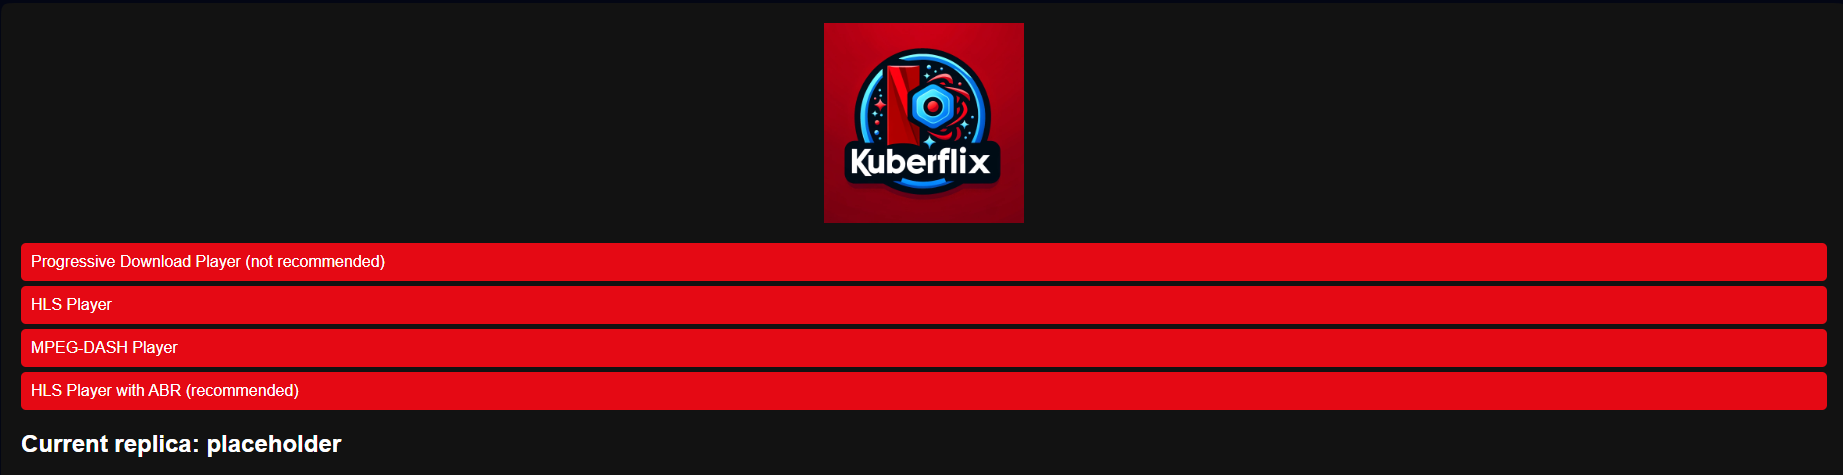
\includegraphics[width=\textwidth]{images/1_home_page.png}
\caption{Home page}
\end{figure}

On the top of the page you can see our logo generated with DALLE 3 AI system.

Under the logo you can see our four players:

\begin{enumerate}
\def\labelenumi{\arabic{enumi}.}
\item
  \texttt{Progressive\ Download\ Player} - default HTML5 player without
  any JavaScript library usage. Keep in mind that default HTML5 player
  does not provide actual streaming but the progressive download
  approach.
\item
  \texttt{HLS\ Player} - player for HLS created using Video.js library.
\item
  \texttt{MPEG-DASH\ Player} - player for MPEG-DASH created using
  Video.js library.
\item
  \texttt{HLS\ Player\ with\ ABR} - player for HLS created using HLS.js
  library along with plyr.io for better visual appearance. This player
  utilize Adaptive Bitrate Streaming, therefore it can change the video
  quality dynamically based on network conditions (bandwith).
\end{enumerate}

Now let's take a look at each player.

\subsubsection{Progressive Download
Player}\label{progressive-download-player}

\begin{figure}[H]
\centering
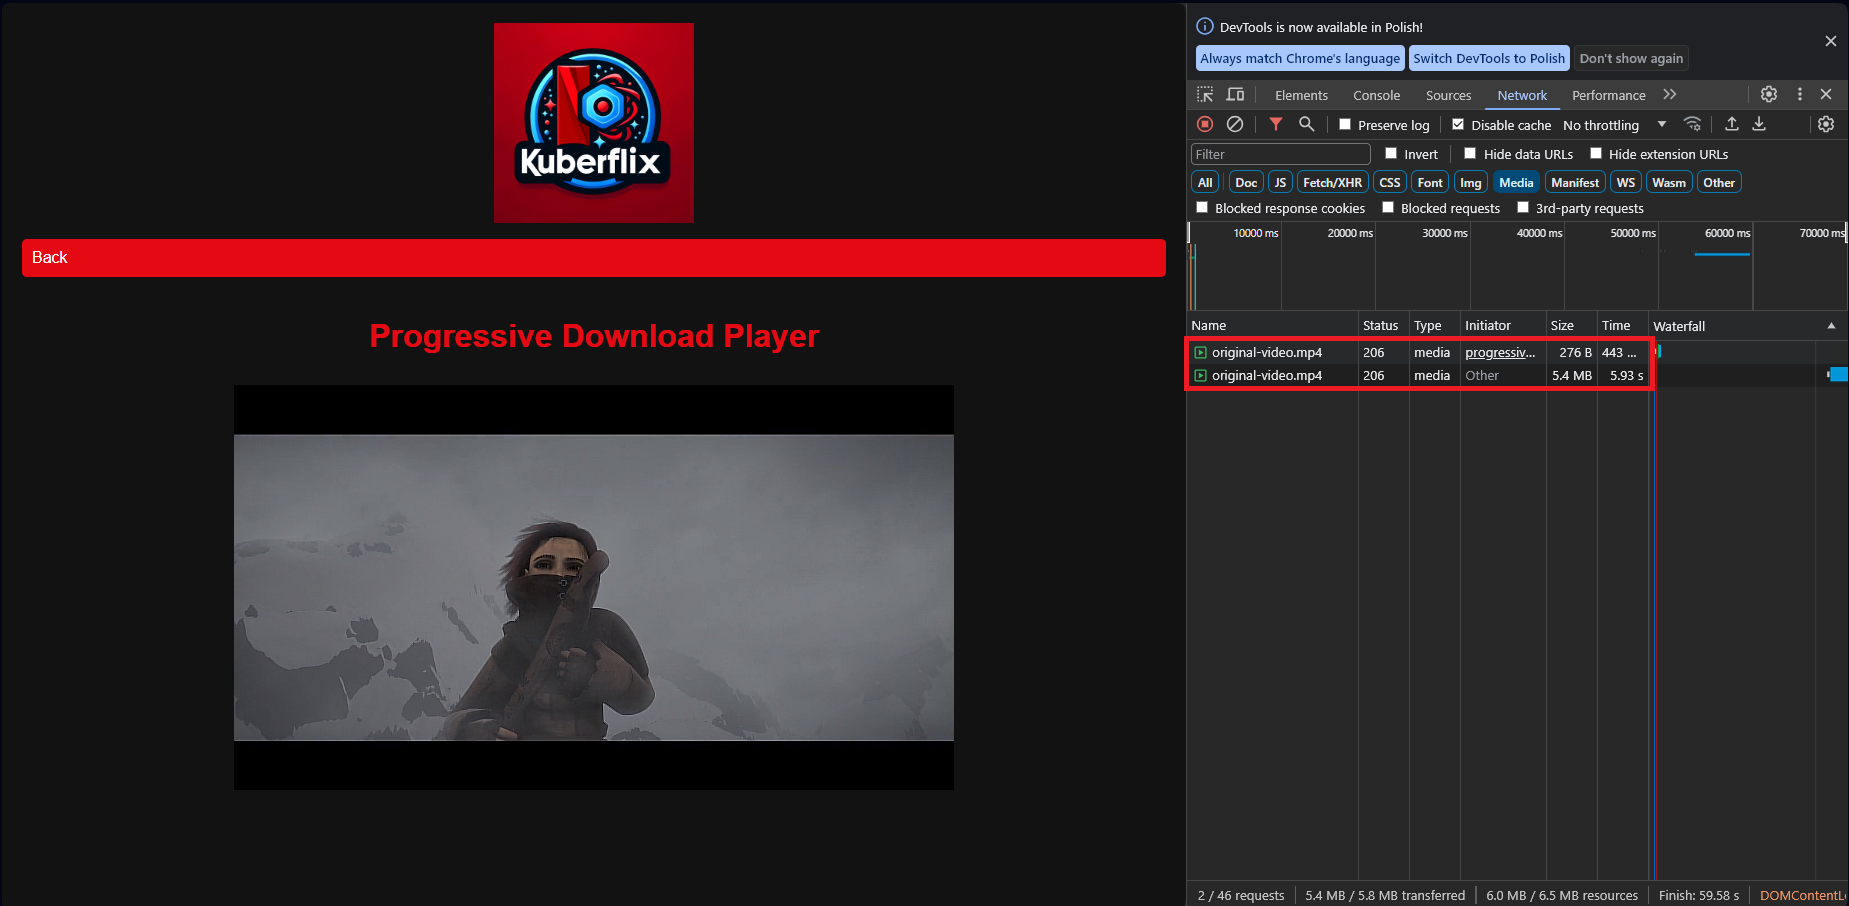
\includegraphics[width=\textwidth]{images/2_progressive_download_player.png}
\caption{Progressive Download Player}
\end{figure}

In Progressive Download Player as the name suggests we simply
progressively download content while watching. In DevTools we can see
appropriate files being downloaded with HTTP 206 Partial Content code.

\subsubsection{HLS Player}\label{hls-player}

\begin{figure}[H]
\centering
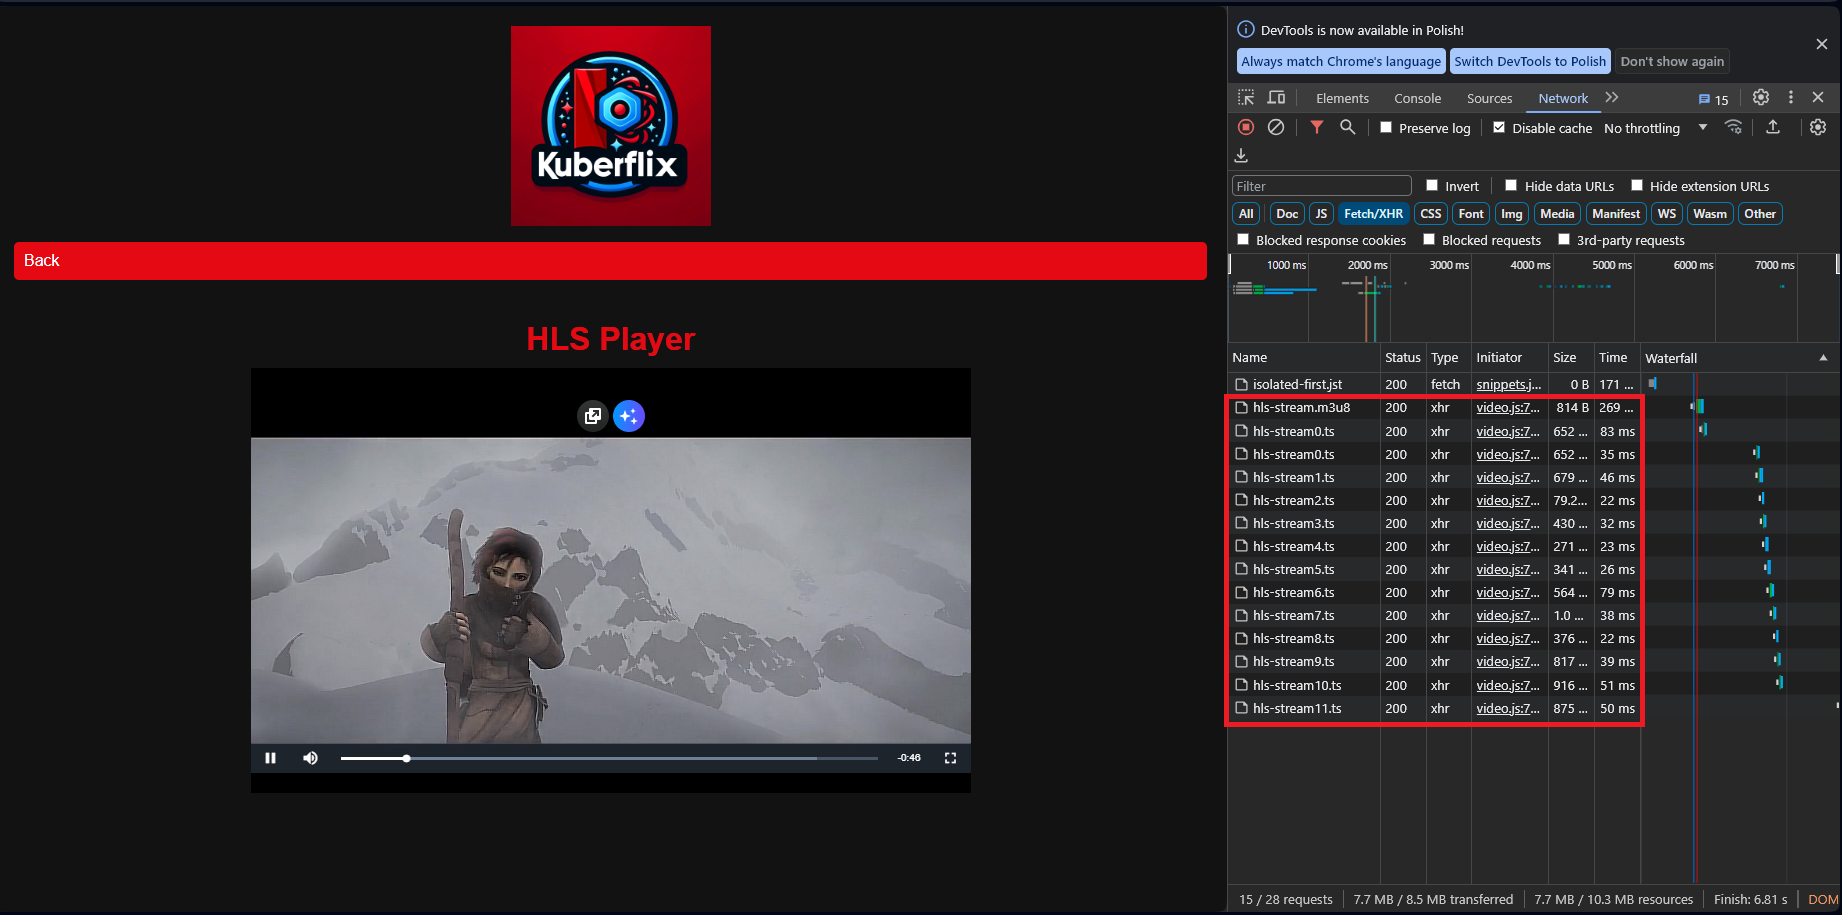
\includegraphics[width=\textwidth]{images/3_hls_player.png}
\caption{HLS Player}
\end{figure}

In HLS player we can see that we properly downloaded .m3u8 playlist and
then we started downloading individual chunks. As was discussed before
each chunk has a few seconds of video and audio and its length may vary
because of key frames distribution. Due to the default Video.js buffer
size we download chunks for next \textasciitilde 30 seconds.

\subsubsection{MPEG-DASH Player}\label{mpeg-dash-player}

\begin{figure}[H]
\centering
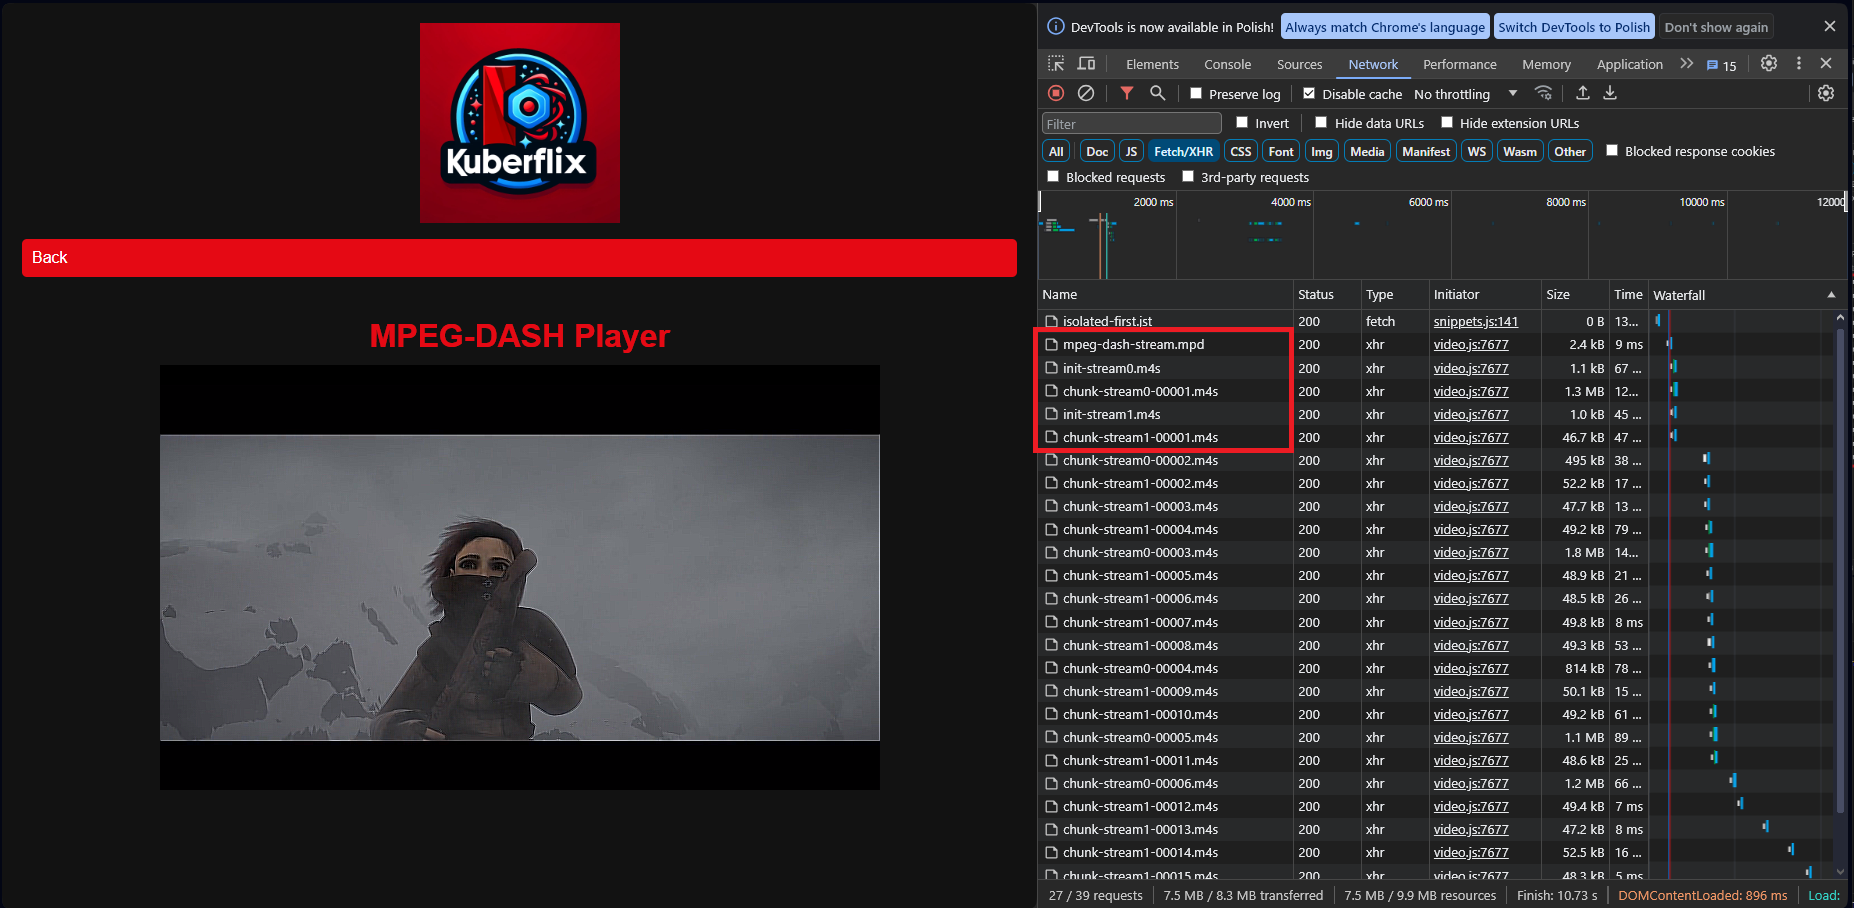
\includegraphics[width=\textwidth]{images/4_mpeg-dash_player.png}
\caption{MPEG-DASH Player}
\end{figure}

In MPEG-DASH player we first download .mpd playlist that contains the
list of all chunks. Then we can see initialization of two streams as
ffmpeg in MPEG-DASH conversion by default separates video and audio for
two streams which can be useful for example in case of multiple language
versions for one video. After initialization we can see downloading
individual chunks of video and audio. Manifest is responsible for the
synchronization between them. MPEG-DASH player is also created in
Video.js and provides \textasciitilde30 seconds buffer.

\subsubsection{HLS Player with ABR}\label{hls-player-with-abr}

Last but not least HLS player with Adaptive Bitrate Streaming (ABR). In
order to show ABR let's first turn on the throttling option in DevTools.
Thanks to it we will be able to show how our application behaves in case
of poor bandwith. It should load the lower quality (144p) of our video.
In order to better visualize bitrate switching I've customized player
buffer to a few seconds instead of default 30s.

\begin{figure}[H]
\centering
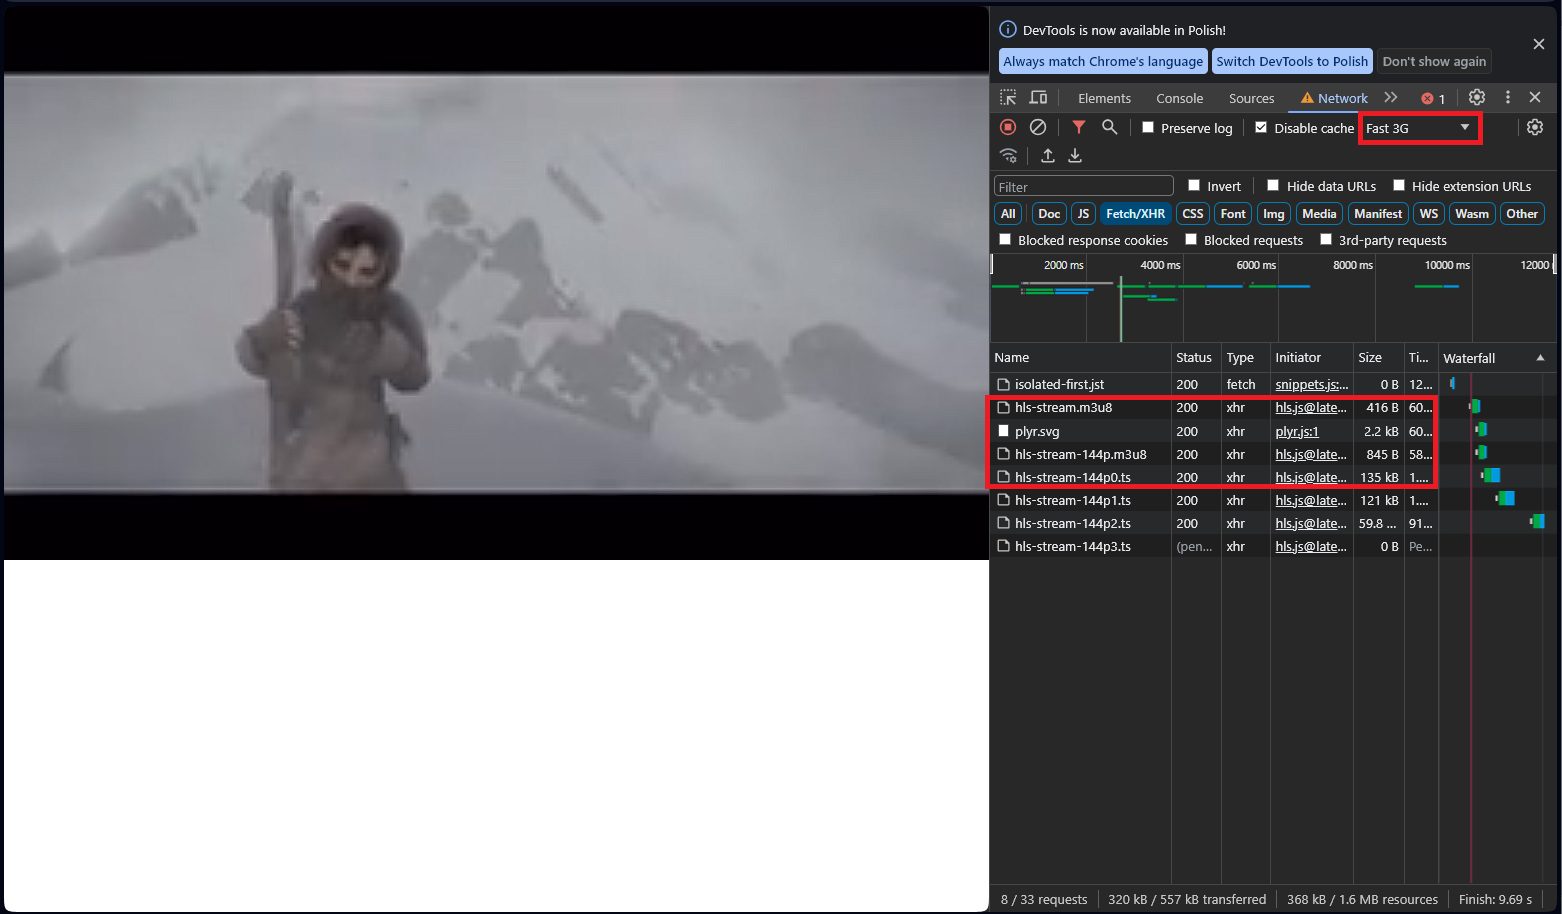
\includegraphics[width=\textwidth]{images/5_hls_player_with_abr_1.png}
\caption{HLS Player with ABR 1}
\end{figure}

As we can see first we download master playlist, which then, based on
our bandwith after applying throttling (see upper right corner) sent us
144p quality playlist and then started to download individual 144p
chunks, which is the desired behavior. We can indeed see that the video
quality is really poor but we wouldn't be able to watch our video
smoothly in good quality.

Now let's turn the throttling down and see if the video quality
improves.

\begin{figure}[H]
\centering
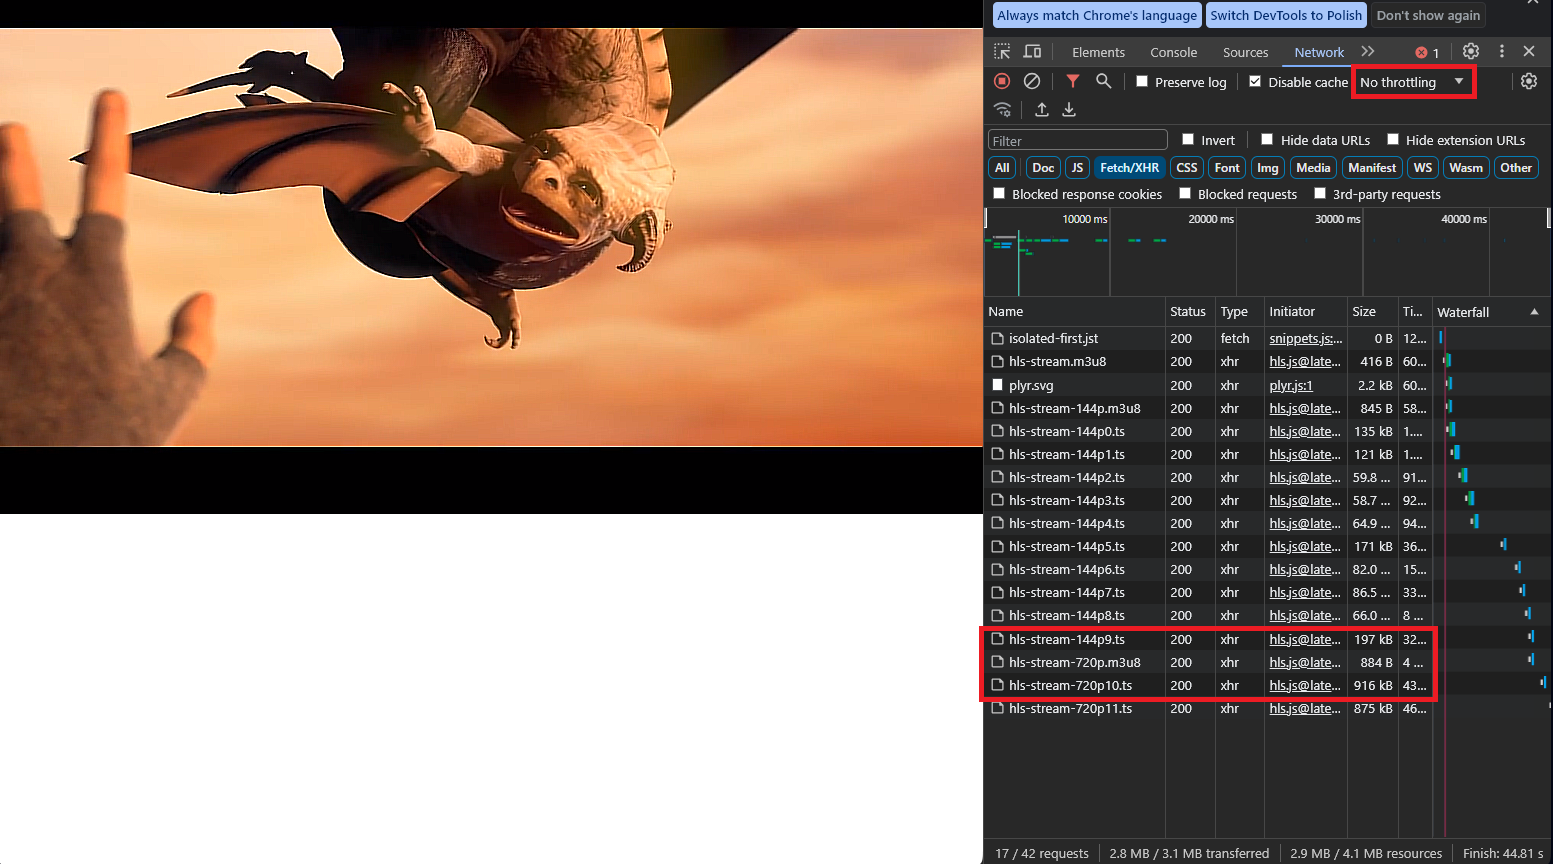
\includegraphics[width=\textwidth]{images/6_hls_player_with_abr_2.png}
\caption{HLS Player with ABR 2}
\end{figure}

As we can see, after removing the throttling video quality improved. We
can see that we downloaded 720p playlist and started downloading
individual 720p chunks, but more importantly the transition between 144p
and 720p was smooth. Keep in mind that it may take some time to adapt to
the throttling manipulation.

Adaptive Bitrate Streaming is a perfect way to provide users smooth
streaming experience without the need of changing the video quality
manually in case of varying network conditions.

\section{Kubernetes}\label{kubernetes}

Kubernetes is a powerful open-source platform for automating the
deployment, scaling, and management of containerized applications. Born
out of the need to efficiently manage container-based workloads at
scale, Kubernetes provides a robust framework for orchestrating and
coordinating the deployment of applications encapsulated in containers.
It allows us to create certain objects with different kinds like
\texttt{Pods}, \texttt{Deployments}, \texttt{Services} or
\texttt{Autoscalers}

\texttt{Pods} in Kubernetes are the smallest deployable units,
representing one or more containers that share the same network
namespace, storage, and IP address. They serve as the basic building
blocks for applications, allowing for efficient deployment, scaling, and
management within the Kubernetes ecosystem.

\texttt{Deployments} in Kubernetes are resources that manage the
deployment and scaling of applications. They use replica sets to
maintain a specified number of \texttt{pod} replicas, supporting rolling
updates and rollbacks for seamless application changes. Deployments
provide a declarative configuration for easy management of the
application's lifecycle, including scaling and updates.

\texttt{Services} in Kubernetes provide a stable endpoint to enable
communication between pods. Acting as an abstraction layer, services
helps with the discovery and load balancing of pods, ensuring seamless
communication within a cluster.

\texttt{Autoscalers} in Kubernetes automatically adjust the number of
pod replicas based on defined metrics or resource utilization. These
dynamic scaling capabilities help optimize performance and ensure
efficient resource usage within the cluster.

To fully demonstrate horizontal streaming autoscaling possibilities we
decided to run our applications on \texttt{minikube}.

\texttt{Minikube} is an open-source tool for running Kubernetes clusters
locally on a single machine. It supports cross-platform use and easy
installation via popular package managers or direct downloads. Minikube
integrates with hypervisors (e.g., VirtualBox, Hyper-V) or can run
Kubernetes nodes as containers using Docker.

To start a local Kubernetes cluster with one node we run a command:

\begin{verbatim}
minikube start
\end{verbatim}

\subsection{Infrastructure}\label{infrastructure}

Main streaming app is created on kubernetes as a Deployment object.
Manifest we use to create it is shown below:

\begin{verbatim}
apiVersion: apps/v1
kind: Deployment
metadata:
  name: streaming-server-deployment
  labels:
    name: streaming-server-deployment
  namespace: streaming-server
spec:
  replicas: 1
  selector:
    matchLabels:
      name: streaming-server-pod
  template:
    metadata:
      labels:
        name: streaming-server-pod
      namespace: streaming-server
    spec:
      restartPolicy: Always
      containers:
        - name: streaming-server-container
          image: streaming-server:latest
          imagePullPolicy: Never
          ports:
            - containerPort: 8080
          resources:
            requests:
              cpu: "10m"
            limits:
              cpu: "50m"
\end{verbatim}

It uses locally built image called \texttt{streaming-server} from

\begin{verbatim}
apps/streaming-server/Dockerfile
\end{verbatim}

By default (After connecting a pod autoscaler to this Deployment - it
changes) only one pod is created with streaming application and it
exposes container port at port :8080.
\newline\texttt{resources: requests: cpu: "10m" limits cpu: "50m"}
set limits at every pod created by Deployment, that he wont be able to
exceed 50 milicores CPU, but it will grant at least 10 milicores CPU per
pod. This limit in combination with \texttt{web-load-simulator} will
help us achieve scalability of pods from 1 to about 5-7 pods.

To allow a communication to this pod we need to create a service, which
will grant us IP and will always connect to the pods created by above
Deployment. Manifest used to create appropiate service is as shown
below:
\begin{verbatim}
apiVersion: v1
kind: Service
metadata:
  name: streaming-server-service
  namespace: streaming-server
spec:
  type: NodePort
  ports:
    - nodePort: 30001
      port: 8080
      targetPort: 8080
  selector:
    name: streaming-server-pod
  sessionAffinity: None
\end{verbatim}
Current configuration allow us to expose Node IP to the external world
that gives us a possibility to reach a streaming app by using web
browser. \texttt{sessionAffinity:\ None} allows us to demonstate that
service is load-balancing the traffic between pods created by Deployment
that service is connected to. After refreshing page we will reach to the
different pod instances.

Every component is stored on separate \texttt{namespace} called
\texttt{streaming-server} which manifest is as simple as:

\begin{verbatim}
apiVersion: v1
kind: Namespace
metadata:
  name: streaming-server
  labels:
    name: streaming-server
\end{verbatim}

Using this helps greatly to separate app's purpose (like
streaming-server, monitoring, metric-server etc.) and manage
applications faster and easier.

\subsection{Horizontal scaling}\label{horizontal-scaling}

To create a Horizontal Pod Autoscaler we are using script with following
command:

{\small
\begin{verbatim}
kubectl autoscale deployment streaming-server-deployment --cpu-percent=50 --min=1 --max=10 -n streaming-server
\end{verbatim}
}

which creates an HPA with following configuration:
\begin{itemize}
  \item Every 15 seconds, check the status of \texttt{deployment} called \texttt{streaming-server-deployment}.
  \item When the deployment's pod count exceeds \texttt{50\%}, scale out.
  \item The minimum and maximum number of pods can be between 1 and 10.
\end{itemize}


To enable the autoscaler getting information about current pod CPU usage
we need to deploy a \texttt{metrics-server} as well.
\texttt{Metrics\ Server} in Kubernetes exposes a simple HTTP API that
allows users to query for real-time metrics data related to the resource
utilization of nodes and pods. This API is essential for applications to
make decisions regarding scaling etc.

We used only essential components stored in

\begin{verbatim}
k8s/metric-server-manifests/components.yaml
\end{verbatim}

from \href{metrics server github}{https://github.com/kubernetes-sigs/metrics-server} where you can
find additional documentation.

To generate a load on our web application we use mentioned before
\texttt{web-load-generator}. It is a single pod deployed manually by the
user on a kubernetes cluster. To do that you need to type
\newline\texttt{kubectl\ apply\ -f\ web-load-generator.yaml} in your terminal.
\newline Generator uses following manifest:
\begin{verbatim}
apiVersion: v1
kind: Pod
metadata:
  name: load-generator
  namespace: streaming-server
spec:
  containers:
  - name: load-generator
    image: busybox:1.28
    command: ["/bin/sh", "-c"]
    args: ["while sleep 0.01; do wget -q -O- streaming-server-service:8080; done"]
  restartPolicy: Never
\end{verbatim}
This pod configuration will create a simple container with busybox image
that will run a script with infinite loop trying to reach our page.
Thanks to the \texttt{service} we dont need to know actual node IP - all
we need to do is use \texttt{streaming-server-service} and Kubernetes
will resolve its IP on its own.

\section*{Bibliography}

\section*{Bibliography}

\begin{thebibliography}{}

\item \url{https://www.iso.org/standard/83314.html}

\item \url{https://www.cloudflare.com/learning/video/what-is-streaming/}

\item \url{https://www.cloudflare.com/learning/video/what-is-mpeg-dash/}

\item \url{https://en.wikipedia.org/wiki/Progressive_download}

\item \url{https://datatracker.ietf.org/doc/html/rfc9113#section-8.1}

\item \url{https://web.archive.org/web/20140821101147/https://www.adobe.com/devnet/rtmp.html}

\item \url{https://www.youtube.com/watch?v=t8ebB9Pxb2s}

\item \url{https://bitmovin.com/wp-content/uploads/2022/12/bitmovin-6th-video-developer-report-2022-2023.pdf}

\item \url{https://www.wowza.com/blog/converting-rtmp-to-hls}

\item \url{https://ffmpeg.org/ffmpeg.html}

\item \url{https://ffmpeg.org/ffmpeg-formats.html#dash-2}

\item \url{https://www.itu.int/ITU-T/recommendations/rec.aspx?rec=14659&lang=en}

\item \url{https://www.rgb.com/h264-profiles}

\item \url{https://www.streamingmedia.com/Articles/ReadArticle.aspx?ArticleID=74735}

\item \url{https://www.cloudflare.com/learning/video/what-is-adaptive-bitrate-streaming/}

\item \url{https://w3techs.com/technologies/overview/web_server}

\item \url{https://docs.nginx.com/nginx/admin-guide/web-server/web-server/}

\item \url{http://nginx.org/en/docs/beginners_guide.html}

\item \url{https://www.w3.org/TR/media-source-2/}

\item \url{https://en.wikipedia.org/wiki/Media_Source_Extensions#Browser_support}

\item \url{https://github.com/video-dev/hls.js/blob/master/docs/API.md}

\item \url{https://docs.videojs.com}

\item \url{https://github.com/sampotts/plyr}

\item \url{https://www.ibm.com/topics/containerization}

\item \url{https://docs.docker.com/get-started/overview/}

\item \url{https://docs.docker.com/engine/reference/builder/}

\item \url{https://kubernetes.io/docs/concepts/}

\item \url{https://minikube.sigs.k8s.io/docs/}

\item \url{https://kubernetes.io/docs/reference/generated/kubectl/kubectl-commands}

\item \url{https://kubernetes.io/docs/tasks/run-application/horizontal-pod-autoscale/}

\item \url{https://github.com/kubernetes-sigs/metrics-server}

\end{thebibliography}


\end{document}